% !TeX spellcheck = it_IT
\newpage
\section{Verifica e validazione}
Verifica e validazione sono attività di \textbf{software quality assurance} e sono parte integrante del processo software da svolgere in ogni fase per confermare che \textbf{processo} e \textbf{prodotto} rispettino i requisiti di qualità.
\begin{center}
	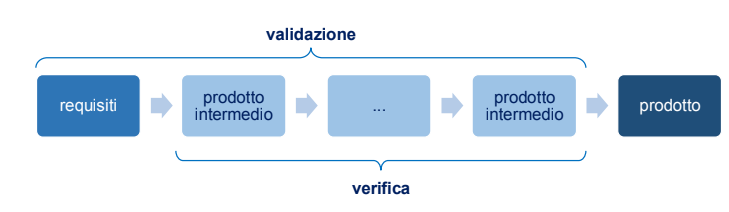
\includegraphics[scale=.4]{vv}
\end{center}
La \textbf{convalida} o validazione risponde alla domanda "Stiamo costruendo il sistema che serve all'utente?" mentre la \textbf{verifica} risponde a "Stiamo costruendo un sistema che rispetta le specifiche?".
\begin{center}
	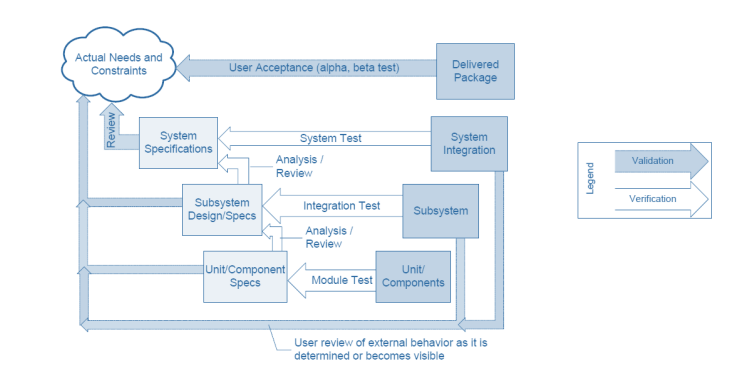
\includegraphics[scale=.5]{vorv}
\end{center}

\subsection{Limiti}
Un risultato fondamentale per la verifica e la validazione è quello dei problemi \textbf{non decidibili}: algoritmi per i quali non esiste alcun algoritmo in grado di dare una risposta in tempo finito su tutte le istanze del problema.

\begin{definition}[Halting problem]
	Non esiste un programma $P$ che per ogni programma $Q$ e input $D$ dice se il programma $Q$ sull'input $D$ termina o meno.
\end{definition}

Un altro esempio di indecidibilità è dire se due programmi, dati gli stessi input, producono lo stesso risultato.

\paragraph{Triple di Hoare}
Una tecnica per la verifica e validazione è tramite le triple di Hoare, basata sulla logica del prim'ordine. Quest'ultima però è \textbf{indecidibile} dato che, data una formula $F$ non esiste un algoritmo per decidere in tempo finito se questa è verificata. È possibile enumerare le formule valide ma non è detto che si dimostri $F$ o $\neg F$.

\subsubsection{Difficoltà}
Le difficoltà principali per la verifica e la validazione sono:
\begin{itemize}
	\item I \textbf{requisiti} di qualità sono \textbf{diversi} tra loro
	\item Un prodotto software è in \textbf{costante evoluzione}
	\item I guasti hanno una distribuzione irregolare
	\item Verifica e validazione sono \textbf{non-lineari}: se una procedura ordina correttamente $X$ elementi non è detto che ne ordini correttamente anche $Y \neq S$
	\item Approcci diversi possono introdurre errori diversi, e.g. il SW distribuito può portare a \textit{deadlock} o \textit{race conditions} mentre quello object-oriented problemi dovuti al \textit{polimorfismo} o al \textit{binding dinamico}
\end{itemize}

\subsection{Progettazione}
I progettisti di questa fase devono:
\begin{itemize}
	\item Scegliere e programmare la giusta combinazione di tecniche per raggiungere il \textbf{livello richiesto di qualità} entro i \textbf{limiti di costo}
	\item Progettare una soluzione specifica che si adatti al \textbf{problema}, ai \textbf{requisiti} e all'\textbf{ambiente di sviluppo}
\end{itemize}

\subsubsection{Quando iniziare e finire}
Verifica e validazione non sono solo una fase finale. Iniziano dallo \textbf{studio di fattibilità}, dove bisogna tenere conto di \textbf{qualità richieste} e \textbf{impatto sul costo} complessivo. Inoltre permettono di svolgere attività correlate alla qualità come:
\begin{itemize}
	\item Analisi del rischio
	\item Definizione delle misure per valutare e controllare la qualità durante le diverse fasi di sviluppo
	\item Valutazione dell'impatto di nuove funzionalità e nuovi requisiti di qualità
	\item Valutazione economica delle attività di controllo della qualità, quali costi e tempi di sviluppo
\end{itemize}
Inoltre continuano anche \textbf{dopo il rilascio} ed includono attività di \textbf{manutenzione}, tra cui:
\begin{itemize}
	\item Analisi delle modifiche ed estensioni
	\item Generazione di nuove suite di test per le funzionalità aggiuntive
	\item Ripetizione dei test per verificare la non regressione delle funzionalità precedenti a seguito di modifiche ed estensioni
	\item Rilevamento ed analisi dei guasti
\end{itemize}

\subsubsection{Quali tecniche}
Non basta una sola tecnica ma è meglio combinarne diverse di analisi e testing, basandosi su diversi aspetti e sulle diverse fasi in cui ci si trova:
\begin{itemize}
	\item \textbf{Efficacia diversa}: per diverse classi di difetto (e.g. analisi statica per identificazione di race conditions)
	\item \textbf{Applicabilità} in \textbf{diverse fasi} del processo di sviluppo (e.g. ispezione per la convalida dei requisiti iniziali e testing per la validazione del prodotto finale)
	\item \textbf{Differenze negli scopi} (e.g. test statistico per misurare l'affidabilità)
	\item \textbf{Compromessi} in termine di costi ed affidabilità (e.g. tecniche costose solo per i requisiti di sicurezza)
\end{itemize}

\subsubsection{Valutazione del prodotto pronto}
Per valutare un prodotto pronto bisogna individuare e definire bene le misure di qualità del software di interesse:
\begin{itemize}
	\item \textbf{Disponibilità} in termini di tempo di esecuzione in rapporto con il tempo in cui il sistema non è disponibile
	\item \textbf{Tempo medio tra i guasti}
	\item \textbf{Affidabilità} misurata come la percentuale di operazioni che terminano con successo
\end{itemize}
Esistono due tipologie di test:
\begin{itemize}
	\item \textbf{Alfa test}: eseguiti da sviluppatori o utenti selezionati, in ambiente controllato ed osservati dall'organizzazione dello sviluppo
	\item \textbf{Beta test}: eseguiti da utenti reali nel loro ambiente e senza interferenze o monitoraggio ravvicinato
\end{itemize}


\subsubsection{Controllare release successive}
Dopo la consegna del prodotto finito ci sono comunque attività che devono essere fatte:
\begin{itemize}
	\item Test ed analisi di codice nuovo o modificato
	\item Ripetizione dei \textbf{test di sistema}
	\item \textbf{Memorizzazione dei bug} trovati
	\item Testi di \textbf{regressione}
	\item Distinzione tra cambiamenti di versione \textit{major} e \textit{minor}
\end{itemize}

\subsubsection{Migliorare il processo}
Per migliorare il processo si devono identificare e rimuovere i punti deboli all'interno del processo di sviluppo e quelli del test e dell'analisi (che non permettono di individuare i primi).

\subsection{Terminologia}
\begin{definition}[Malfunzionamento]
	Il sistema SW a runtime non si comporta secondo le specifiche. Ha natura \textbf{dinamica} e può essere osservato solo mediante esecuzione. È causato da uno o più difetti.
\end{definition}
\begin{definition}[Difetto]
	Anomalia, bug o fault nel codice del sistema SW. Appartiene alla struttura statica del programma. L'atto di correzione è definito \textbf{debugging} o \textbf{bug fixing}. Può causare uno o più malfunzionamenti e se non ne causa si dice che è \textbf{latente} (e.g. in un flusso che non viene quasi mai eseguito o difetti che si annullano a vicenda).
\end{definition}

\begin{definition}[Errore]
	È la causa del difetto. Un errore umano nella comprensione o risoluzione dei problemi o nell'uso di strumenti.
\end{definition}

\subsection{Verifica statica}
La verifica statica non prevede l'esecuzione del programma e si divide in due tipi di metodi:
\begin{itemize}
	\item \textbf{Manuali}: basati sulla \textit{desk-check} (lettura del codice). Sono i più comuni e più o meno formalmente documentati.
	\item \textbf{Formali} o supportati da \textbf{strumenti}:
	\begin{itemize}
		\item Model checking
		\item Esecuzione simbolica
		\item Interpretazione astratta
		\item Theorem proving
	\end{itemize}
\end{itemize}

\subsubsection{Desk check}
Il desk-check è l'analisi manuale di programmi software volta a capire cosa facciano e/o ad identificare errori logici che potrebbero occorrere durante la loro esecuzione. Esistono due metodologie \textbf{pratiche} (lettura del codice e dipendenti dall'esperienza) e \textbf{complementari} tra loro: \textit{inspection} e \textit{walkthrough}.
\paragraph{Inspection} Si esegue una lettura mirata del codice guidata da una checklist. L'biettivo è di rivelare la presenza di difetti focalizzando la ricerca su aspetti ben definiti (error guessing) (e.g. off-by-one error). La ricerca viene portata avanti dagli \textbf{ispettori}. Si divide in quattro fasi:
\begin{enumerate}
	\item \textbf{Pianificazione}
	\item Definizione della \textbf{checklist}. Sono frutto dell'esperienza degli ispettori. Tipicamente contengono aspetti che non sono controllabili in maniera automatica e sono aggiornate ad ogni iterazione.
	\item \textbf{Lettura} del codice
	\item \textbf{Correzione} dei difetti
\end{enumerate}

\paragraph{Walkthrough} Si esegue una lettura critica del codice con l'obiettivo di rivelare la presenza di difetti percorrendo il codice e simulandone l'esecuzione. È eseguita da gruppi misti di \textit{ispettori} e programmatori. È più completo dell'inspection ma meno rapido. Si divide in tre fasi:
\begin{enumerate}
	\item \textbf{Pianificazione}
	\item \textbf{Lettura} del codice
	\item \textbf{Correzione} dei difetti
\end{enumerate}

Il desk-check è \textbf{pratico} ed \textbf{intuitivo}, rendendolo ideale per alcune caratteristiche di qualità. Inoltre \textbf{conviene economicamente}: i costi dipendono dalla dimensione del codice e sono quindi bassi per quanto riguarda l'infrastruttura. Permette una buona prevedibilità dei risultati.

\subsubsection{Metodi formali}
I metodi formali sono tecniche basate sulla dimostrazione formale di correttezza di un modello finito (che ha dimostrazione possibile) e istanziazione del modello.
\begin{example}[Two-phase locking]
	Il protocollo two-phase locking, una volta dimostrato corretto e istanziato correttamente, garantisce assenza di malfunzionamenti dovuti alla race condition. Allo stesso tempo però ci sono applicazioni che non lo usano ma che sono comunque corrette e bisogna anche dimostrare che il programma applichi il protocollo correttamente (comunque più facile che provare l'assenza di malfunzionamenti in generale).
\end{example}
Esempi di metodi formali sono le \textbf{triple di Hoare}, il \textbf{B method} e il \textbf{model checking.}
\begin{figure}[!h]
	\hfill
	\subfigure[Triple di Hoare]{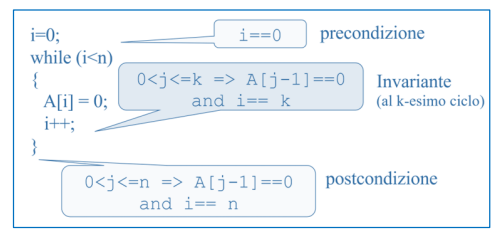
\includegraphics[width=7cm]{hoare}}
	\hfill
	\subfigure[Model checking]{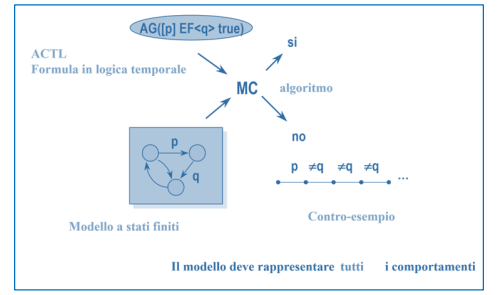
\includegraphics[width=7cm]{modelcheck}}
\end{figure}